\chapter{Considered Deployment Schemes}
\label{sec:considered_deployment_schemes}
In addition to the deployment schemes outlined in \ref{sec:greedy_deployment},
\ref{sec:random_deployment}, and \ref{sec:initially_random_greedy}, this chapter outlines others not included in the final analysis. I examined these schemes for their potential to capture the complexity of the deployment problem but were ultimately not included due to the egregious nature of approximation required to implement or the lack of a clear benefit over the other schemes for the questions explored in this work.

\section{Capped Deployment}
\label{sec:capped_deployment}
This scheme places a constant limit on the number of specific reactors deployed
at any given time step. This is a simple way to model aggregate supply chain
constraints that could limit vendors from deploying reactors freely. With the
right constraints, this scheme would better succeed at roughly incorporating
the limits of a workforce over a short to medium time scale. This thesis does not implement the capped deployment scheme as workforce constraints are outside the scope.

To use this deployment scheme, a user needs to understand the supply chain constraints that will limit the deployment of the reactors they are deploying. Figure \ref{fig:cap_diagram} illustrates the defining steps of the capped deployment scheme. The main loop in the logic is consistent with the greedy deployment scheme but adds a check to see if the current deployment exceeds the limit on that reactor. If it does, the reactor is removed from the list of reactors to be deployed in that time step.

\begin{figure}[H]
    \centering
    \begin{tikzpicture}[node distance = 2.5cm, auto]
        % Place nodes
        \node [block] (init) {\textbf{Initialize demand.}};
        \node [block, below of=init] (check) {\textbf{Is there demand?}};
        \node [block, below of=check, node distance=3cm] (evaluate) {\textbf{Deploy the largest capacity capped reactor below demand.}};
        \node [block, below of=evaluate, node distance=3cm] (cap) {\textbf{Does this deployment meet a cap?}};
        \node [block, right of=cap, node distance=4cm] (remove) {\textbf{Remove reactor from list.}};
        \node [block, right of=remove, node distance=4cm] (update) {\textbf{Update demand.}};
        \node [block, left of=check, node distance=4cm] (stop) {\textbf{Next time step.}};
        % Draw edges
        \path [line, line width=0.6mm] (init) -- (check);
        \path [line, line width=0.6mm] (check) -- node {\textbf{Yes}} (evaluate);
        \path [line, line width=0.6mm] (evaluate) -- (cap);
        \path [line, line width=0.6mm] (check) -- node {\textbf{No}}(stop);
        \draw[->, line width=0.6mm] (update) edge[bend right=45] node[right]{} (check);
        \draw [line, line width=0.6mm] (cap) edge[bend right=45] node {\textbf{No}} (update);
        \path[line, line width=0.6mm] (cap) -- node {\textbf{Yes}} (remove);
        \path[line, line width=0.6mm] (remove) -- (update);
    \end{tikzpicture}
    \caption{Capped deployment diagram.}
    \label{fig:cap_diagram}
\end{figure}

% \begin{figure}[H]
%     \centering
%     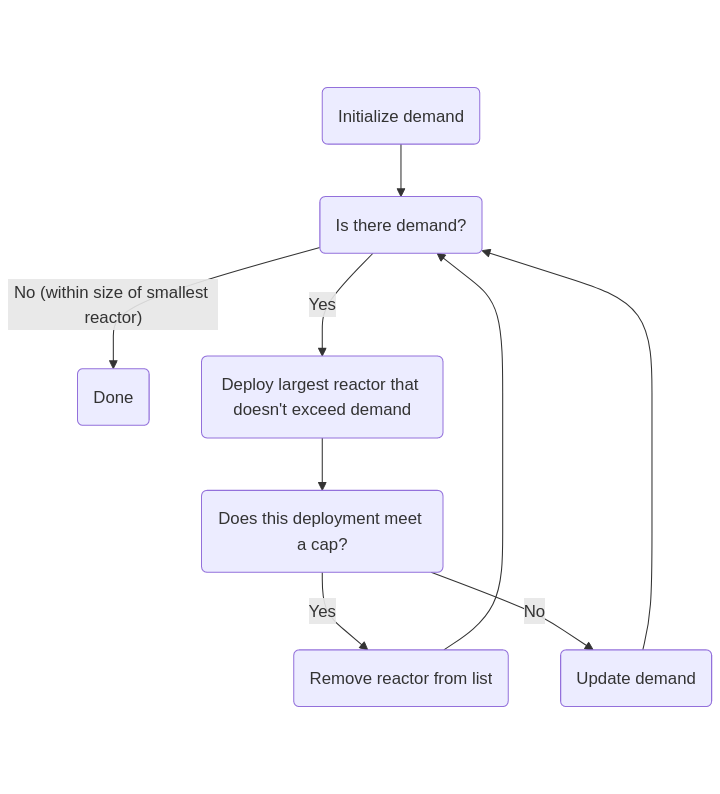
\includegraphics[scale=0.4]{images/schemes/cap_diagram.png}
%     \caption{Capped deployment diagram.}
%     \label{fig:cap_diagram}
% \end{figure}

The realism of this deployment scheme mirrors some elements of the
pre-determined distribution (this is a flat distribution after all), but the
cap is a less granular way to account for supply chain constraints. This scheme
is most useful for scenarios or timescales where there is a known limit on the
workforce. The unrealistic element of this deployment scheme comes from two
places: 1) the current implementation requires one reactor to be unrestrained
(preferably the smallest reactor from the deployment standpoint); 2) the cap is
a flat distribution, which is not a realistic representation of the supply
chain constraints for most technologies.

When the unconstrained reactor is not the smallest power reactor, this scheme
will fall below demand moreso than when the unconstrained reactor is the
smallest in power. This scheme has the potential to overperform by one reactor
in the case where the unconstrained reactor is the smallest in power as it can
over-deploy by one reactor's capacity in that case.

\section{Pre-Determined Distribution Deployment}
\label{sec:pre_determined_distribution_deployment}
This deployment scheme allows users to incorporate the projections and
commitments of ratepayers and utilities by setting a distribution over the
simulation time. In this scheme, the distribution serves as a cap to the
number of reactors deployed in a time step, and preferentially
deploys reactors first to meet those caps. After completion, it deploys the
remaining reactors without caps to meet the demand. In this way, it allows a user to incorporate knowledge of supply chain constraints for specific technologies without modeling the supply chain in detail.

To use this deployment scheme, a user needs some idea of the distribution of reactors deployed over the simulation time. Figure \ref{fig:pre_det_diagram} illustrates the defining steps of the pre-determined distribution deployment scheme. The main loop in the logic is consistent with the greedy deployment scheme but adds a check to see if the current deployment exceeds the limit on that reactor. If it does, the scheme removes the reactor from the list of deployable reactors in that time step. This scheme varies from the capped deployment scheme in that the distribution is not flat, but a more granular distribution that varies by year.

\begin{figure}[H]
    \centering
    \begin{tikzpicture}[node distance = 2.5cm, auto]
        % Place nodes
        \node [block] (init) {\textbf{Initialize demand.}};
        \node [block, below of=init] (check) {\textbf{Is there demand?}};
        \node [block, below of=check, node distance=3cm] (evaluate) {\textbf{Deploy the largest capacity reactor below demand.}};
        \node [block, below of=evaluate, node distance=2.5cm] (cap) {\textbf{Does it meet a limit?}};
        \node [block, right of=cap, node distance=4cm] (remove) {\textbf{Remove reactor from list.}};
        \node [block, right of=remove, node distance=4cm] (update) {\textbf{Update demand.}};
        \node [block, left of=check, node distance=4cm] (stop) {\textbf{Next time step.}};
        % Draw edges
        \path [line, line width=0.6mm] (init) -- (check);
        \path [line, line width=0.6mm] (check) -- node {\textbf{Yes}} (evaluate);
        \path [line, line width=0.6mm] (evaluate) -- (cap);
        \path [line, line width=0.6mm] (check) -- node {\textbf{No}}(stop);
        \draw[->, line width=0.6mm] (update) edge[bend right=45] node[right]{} (check);
        \draw [line, line width=0.6mm] (cap) edge[bend right=45] node {\textbf{No}} (update);
        \path[line, line width=0.6mm] (cap) -- node {\textbf{Yes}} (remove);
        \path[line, line width=0.6mm] (remove) -- (update);
    \end{tikzpicture}
    \caption{Pre-determined distribution deployment diagram.}
    \label{fig:pre_det_diagram}
\end{figure}

% \begin{figure}[H]
%     \centering
%     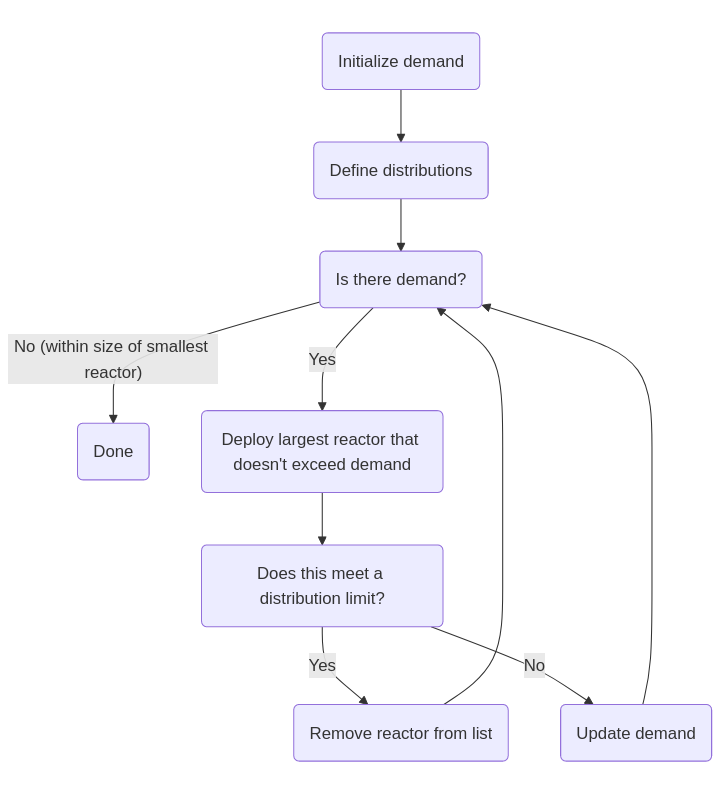
\includegraphics[scale=0.4]{images/schemes/pre_det_diagram.png}
%     \caption{Pre-determined distribution deployment diagram.}
%     \label{fig:pre_det_diagram}
% \end{figure}

The realism of this deployment scheme mirrors some elements of the capped
deployment, but the distribution is a more granular way to account for supply
chain constraints. This scheme is most useful when there are known commitments
to specific technologies. It allows the user to indirectly incorporate the
evolution of supply chains or workforce constraints over time, and to
explicitly incorporate decisions from individual actors. If a user established
the nuances of the supply chain constraints in other work, it could be
incorporated through this scheme. Under and over-performance of this scheme is
difficult to predict, as it depends on the distribution of reactors over time.